多語言語音辨識系統中,問題核心旨在如何利用其他語言的豐富資料輔助彼此學習,達到相同資料量卻比較好的結果。本章先簡介評估多語言辨識系統情境的方法,接著由粗糙到細緻的順序,分別介紹基於國際音標、基於狀態合併以及基於模型共享的三種不同層級多語言語音辨識系統架構。

\section{評估多語言語音辨識系統}
單語言語音辨識情境下,比較系統辨識結果以及正確詞序列,可以計算該語言的詞錯誤率。如果在使用某種方法與架構後,使得詞錯誤率比起基準實驗下降,則可以合理推斷該方法有幫助於語音辨識系統。然評估多語言辨識系統時,下列三種情形會發生:
\begin{itemize}
 \itemsep -2pt
 \item 每個語言的詞錯誤率,都比相應語言的基準實驗低。
 \item 每個語言的詞錯誤率,都比相應語言的基準實驗高。
 \item 有些語言的詞錯誤率,比相應語言的基準實驗高,但有些則比較低。
\end{itemize}
因應不同語言的特性,不同的方法可能有較適用的語言。上述的前兩種情形,評估時與單語言語音辨識系統無異。然第三種情形,也是評估多語言語音辨識系統時最常見的情形,卻會因為不同語言的進退步比例不同,而無法單純使用詞錯誤率清楚呈現進退步狀況。

因此,本論文在評估多語言語音辨識系統時,除了呈現各語言的詞錯誤率以外,同時會呈現多語言的平均詞錯誤率比(Average WER Ratio, AWERR),為每個語言的詞誤比(WERR)的幾何平均,公式如下:

\begin{equation}\label{eq:AWERR}
AWERR = ( \prod_{l=1}^{L} {WERR^{(l)}} )^{\frac{1}{L}}
\end{equation}
\begin{equation}\label{eq:WERR}
WERR^{(l)} = \frac{WER_{target}^{(l)}}{WER_{reference}^{(l)}}
\end{equation}

其中小寫$l$代表的是某個語言,$L$為語言總共的數量,在本論文為4個語言。$WER_{target}^{(l)}$為語言$l$的某種情境的詞錯誤率,$WER_{reference}^{(l)}$為語言$l$的基準實驗詞錯誤率。

AWERR是詞誤比的平均,因此越低的AWERR,則表示該方法對於多語言辨識系統的整體詞錯誤率下降越多。

使用AWERR作為評估時,須注意AWERR對於原本基準實驗中比較較好的語言比較敏感,因為在公式\ref{eq:WERR}中基準實驗的結果放在分母。且AWERR是使用幾何平均,而非算術平均,對於詞錯誤率的降低比較敏感,對於詞錯誤率的提昇比較不敏感。

倘若詞錯誤率在大部份語言中降低的比較多,在少部份語言降低的比較少甚至還有些微提昇時,仍可視為該方法能夠幫助多語言語音辨識系統,但對於該語言的幫助較小。


\section{基於國際音標進行音素合併}

國際音標基於人類發音的方式與發音部位的位置,將不同音素合併在同一個國際音標中,直觀上而言,人耳聽起來極為接近的聲音,就會在國際音標上被分類在同一個符號裡,藉由將相近的發音單位合併,可以增加聲學模型的訓練資料量,使用其他語言的資料輔助學習,學習到橫跨多語言的資訊。

\subsection{音素合併表}
本論文使用的四個語言,皆有語言學家標示出的音素集(Phone set)以及每個音素對應的國際音標(IPA)。如果兩個不同語言的音素被標記為相同的國際音標,則代表語言學家認為其發音部位跟聲音相似,且人耳幾乎無法辨識出差異。理論上,語音辨識系統應該可以把兩個音素辨識為同一個發音單位。

\begin{table}
\centering
\renewcommand{\arraystretch}{0.5}
\begin{tabular}{|c|cccc|}
\hline
 IPA & 西語 & 捷克 & 法語 & 德語 \\
\hline
 sil  & sil & sil & sil  & sil \\ 
   a  &  a  &  a  & a    &  a  \\
  a+  & a+  &     &      &     \\
  A~  &     &     & A~   &     \\
  ae  &     &  e  & E    &  ae \\
  AE  &     &     & AE   &     \\
  aeU &     &  ew &      &     \\
  aI  & aI  &     &      &  aI \\
  al  &     &  aa &      &  al \\
  atu &     &     &      & atu \\
  aU  & aU  &  aw &      &  aU \\
  b   &  b  &   b &  B   &   b \\
  C   &     &     &      &   C \\
  d   &  d  &   d &  D   &   d \\
  D   &  D  &     &      &     \\
  dj  &     &  dj &      &     \\
  e   &  e  &     & e    &   e \\
  e+  &  e+ &     &      &     \\
  E~  &     &     & E~   &     \\
  eI  & eI  &     &      &     \\
  el  &     &  ee &      &   el \\
  etu &     &     & AX   &  etu \\
  eU  & eU  &     &      &     \\
  EU  &     &     & EU   &     \\
  f   &  f  &  f  & F    &   f  \\
  g   &  g  &  g  & G    &   g  \\
  G   &  G  &     &      &     \\
  h   &     &     & h    &   h  \\
  h~  &     &  h  &      &     \\
  H   &     &     & H    &     \\
  i   &  i  &     & i    &   i  \\
  i+  &  i+ &     &      &     \\
  I   &     &  i  &      &     \\
  il  &     & ii  &      &   il \\
  j   &  j  &  j  & J    &    j \\
  k   &  k  &  k  & K    &    k \\
  l   &  l  &  l  & L    &    l \\
  L   &  L  &     &      &      \\
  m   &  m  & m,mg & M   &    m \\
  n   &  n  &  n   & N   &    n \\
\hline
\end{tabular}
\begin{tabular}{|c|cccc|}
\hline
 IPA & 西語 & 捷克 & 法語 & 德語 \\
\hline
  n~  &  n~ &  nj  & NJ  &      \\
  N   &  ng &      & NG  &      \\
  ng  &     &  ng  &     &   ng \\
  o   &  o  &   o & o    &   o  \\
  o~  &     &     & o~   &      \\
  o+  &  o+ &     &      &      \\
  O   &     &     & O    &      \\
  oe  &     &     & OE   &   oe \\
  oe~ &     &     & OE~  &      \\
  oel &     &     &      &  oel \\
  oI  &  oI &     &      &      \\
  Oi  &     &     &     &  eU \\
  ol  &     & oo  &     &  ol \\
  oU  &     & ow  &     &     \\
  p   &  p  &  p  & P   &   p \\
  r   &  r  &  r  &     &   r \\
  R   &     &     & R   &     \\
  rf  & rf  &     &     &     \\
  rsh &     & rsh &     &     \\
  rzh &     & rzh &     &     \\
  s   &  s  &  s  & S   &   s \\
  S   &     & sh  & SH  &   S \\
  t   &  t  &  t  & T   &   t \\
  T   &  T  &     &     &     \\
  tj  &     & tj  &     &     \\
  ts  &     &  c  &     &  ts \\
  tS  &  tS & ch  &     &     \\
  u   &  u  &  u  & u   &   u \\
  u+  &  u+ &     &     &     \\
  ue  &     &     &     &  ue \\
  uel &     &     &     & uel \\
  ul  &     & uu  &     &  ul \\
  v   &     &  v  & V   &   v \\
  V   &  V  &     &     &     \\
  w   &  w  &     &     &     \\
  W   &     &     & W   &     \\
  x   &  x  &  x  &     &   x \\
  y   &     &     & y   &     \\
  z   &  z  &  z  & Z   &     \\
  Z   &     &     & ZH  &     \\
\hline
\end{tabular}
\caption{西班牙語、捷克語、法語、德語的音素與對應的國際音標表}
\label{table:GP_IPA_mapping}
\end{table}

表\ref{table:GP_IPA_mapping}為本論文使用的四個語言的音素與國際音標對應表。根據這個表格,可以將特定語言的辭典轉化為以國際音標為單位建成的辭典,並且將四個語言的資料混雜,重新訓練多語言語音辨識系統的架構,如圖\ref{fig:chap4_IPA_merged}。

\begin{figure}[!h]
\centering
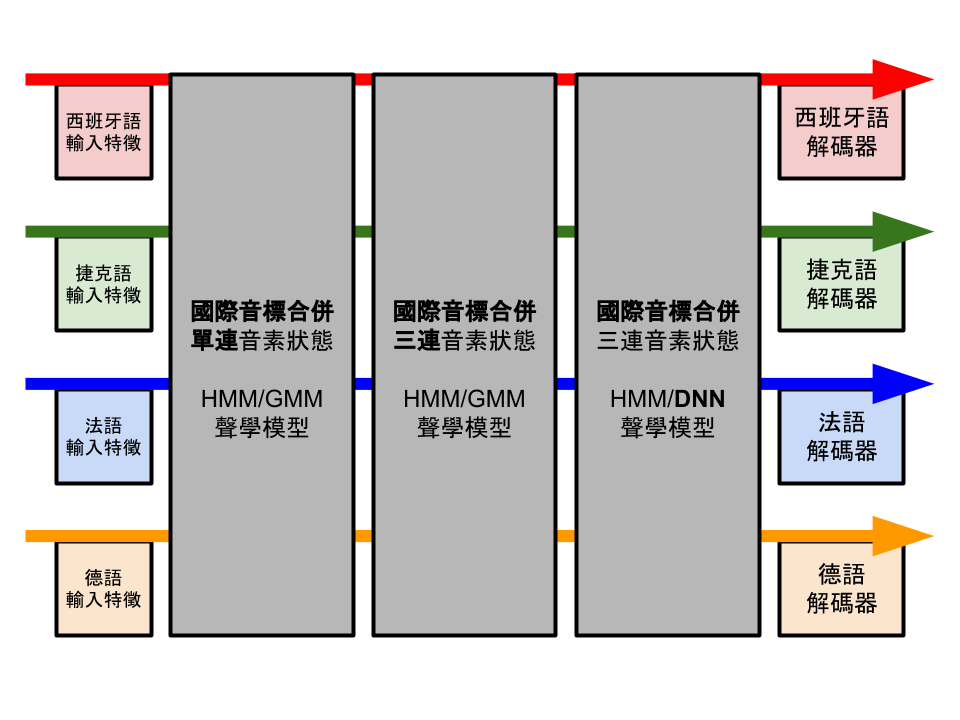
\includegraphics[scale=0.4]{images/chap4_IPA_merged.png}
\caption{基於國際音標合併音素集的西班牙語、捷克語、法語、德語多語音辨識系統}
\label{fig:chap4_IPA_merged}
\end{figure}

圖\ref{fig:chap4_IPA_merged}中,四個語言的資料混合起來,從底層重新開始訓練單連音素HMM/GMM聲學模型、三連音素HMM/GMM聲學模型、三連音素深層類神經網路聲學模型。評估時,四個語言仍然會與相應的辭典以及語言模型結合,形成特定語言的解碼器,產生辨識結果。

\subsection{實驗結果與分析}

\begin{table}[htbp]
%\resizebox{\columnwidth}{!}{
\centering
\begin{tabular}{|c>{\columncolor{red!20}}c>{\columncolor{green!20}}c>{\columncolor{blue!20}}c>{\columncolor{yellow!20}}c>{\columncolor{gray}}cc|}
\hline
 方法 & 西語 & 捷克 & 法語 & 德語 & AWERR & 參數數量 \\
\hline
  單語言基準實驗 & 8.74\% & 18.16\% & 17.43\% & 15.85\% & 100\% & 75.6M \\
\hline
  6073個狀態 & 10.03\% & 18.89\% & 18.78\% & 17.27\% & 108.8\% & 26.3M \\
\hline
  7633個狀態 & 9.53\% & 19.13\% & 18.60\% & 17.08\%  & 107.2\% & 29.5M\\
\hline
  8010個狀態 & 9.51\% & 18.80\% & 18.56\% & 16.78\%  & 106.2\% & 30.3M\\
\hline
\end{tabular}
\caption{基於國際音標合併的多語言辨識系統詞錯誤率,與單語言基準實驗比較。表中的深層類神經網路模型都是4層寬度2048神經元,使用S型函數且未使用丟棄演算法。合併後的模型參數數量減少許多,是因為四個語言間共用了大量的深層類神經網路參數。}
\label{table:chap4_IPA_merged}
\end{table}

表\ref{table:chap4_IPA_merged}為辨識結果評估,無論是哪一個語言,詞錯誤率都比單語言的基準實驗高,因此AWERR是大於100\%的數字。基於國際音標合併多語言的音素集,顯然沒有幫助個別語言的詞錯誤率下降,各個語言使用自己的單語言辨識系統結果都較好。

分析實驗結果,推斷可能的原因為:
\begin{itemize}
 \itemsep -2pt
  \item 將各個語言的音素集合併形成全域音素集後,總計會有80個音素,使得訓練考量前後文相依的三連音素聲學模型時,模型複雜度三次方上升,所需的訓練資料量嚴重不足,使得聲學模型無法訓練完全。
  \item 有些音素獨立於其他音素之外,不會與其他語言共用的特定語言音素,合併後情況依然。然而在訓練深層類神經網路時,該資料量相較於整體資料量的比例會因此下降,造成事前機率過低,不容易被辨識出來。
  \item 即便被分類在同樣的國際音標符號,不同語言的音素仍然會有差異。被標成同樣IPA符號的音素,有大部分於人耳聽起來根本不同,合併其實沒有互相傳授跨語言知識的意義。
\end{itemize}

然而,考量到深層類神經網路模型的參數數量時,會發現這個方法具有有損壓縮(Lossy compression)的效果。基於國際音標合併音素的多語言語音辨識系統,會在不同語言中共享深層類神經網路模型,比起單語言語音辨識系統,能夠節省59\% 到 65\%的模型參數數量,但會增加6.2\% 到 8.8\%的AWERR。隨著參數數量增加,壓縮效果減少,辨識結果相對變好,有折衷(trade-off)空間。

\section{基於資料混淆矩陣的音素狀態合併}
上節基於國際音標合併音素,是根據人耳對於發音單位的鑑別力,來進行合併。然在機器層面上,音素層級的發音單位太過粗糙。本論文著眼於這個點,探討一個更細緻的合併方法,也就是本節資料導向(Data-driven)以混淆矩陣(Confusion Matrix)的三連音素狀態合併。


\subsection{混淆矩陣}
三連音素狀態,是在聲學模型訓練過程中分割單連音素狀態而成的更細緻發音單位,本身就是來自於資料特性所形成的,因此缺少了語言學家的標定,無法藉由知識標記不同狀態的相似性。因此,本論文借助資料導向(Data-driven)的方式,建立混淆矩陣(Confusion Matrix, CM)來找出相近的三連音素狀態進行合併。

\begin{figure}[!h]
\centering
\subfloat[][對稱性] {
    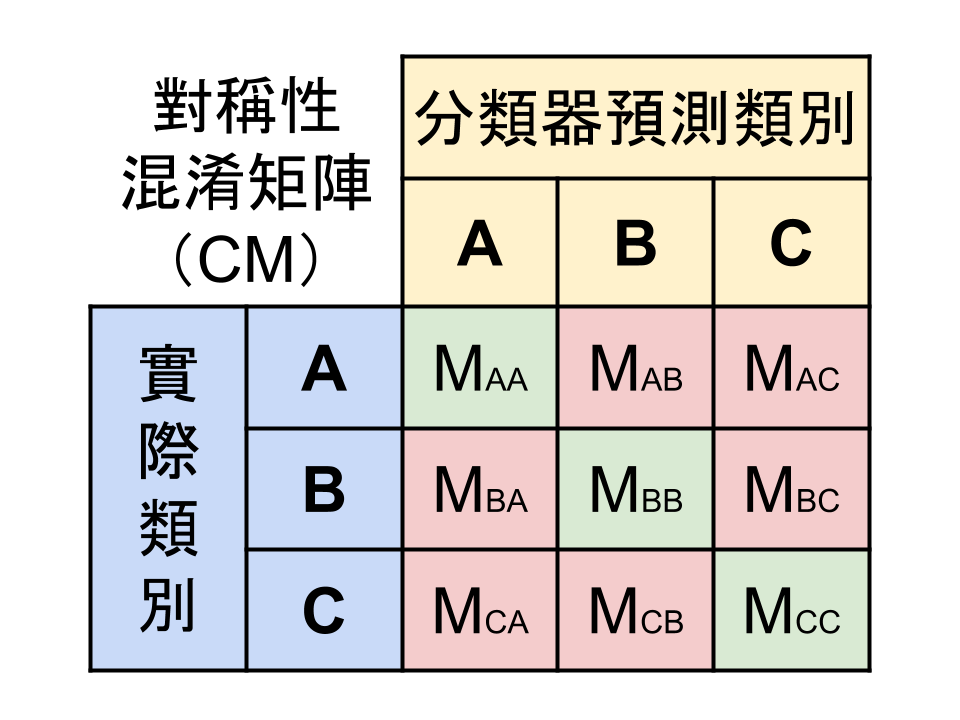
\includegraphics[scale=0.18]{images/chap4_CM.png}
    \label{fig:chap4_CM}
}
\subfloat[][非對稱性] {
    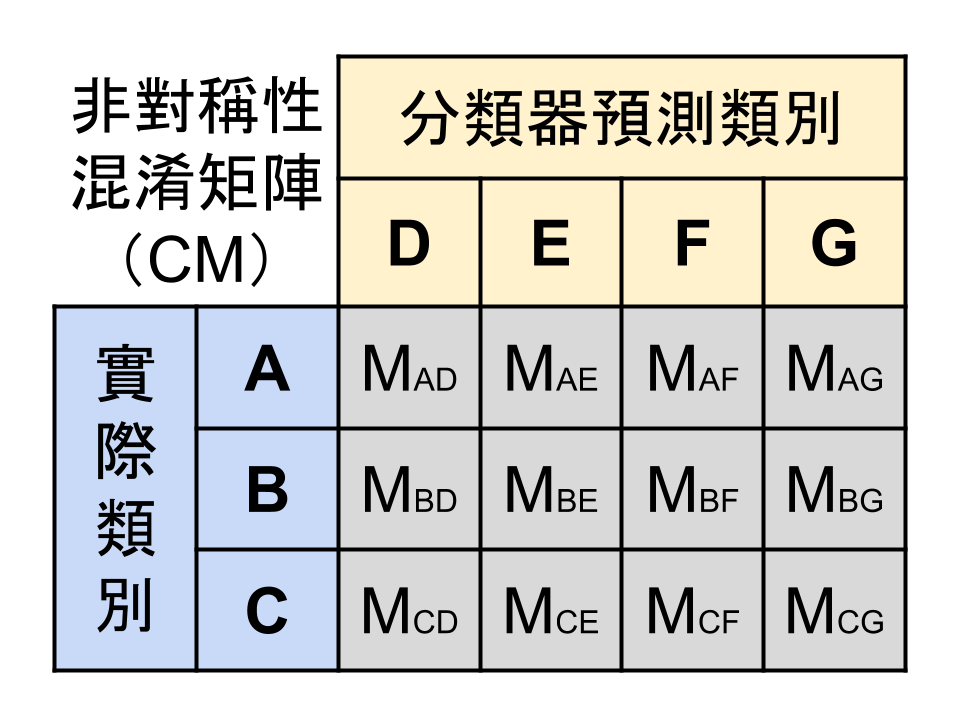
\includegraphics[scale=0.18]{images/chap4_CM_asymm.png}
    \label{fig:chap4_CM_asymm}
}
\caption{典型的混淆矩陣示意圖}
\end{figure}

混淆矩陣(Confusion Matrix),是衡量分類器測試結果時,輔助呈現的一張矩陣式表格。如圖\ref{fig:chap4_CM}中,每一列是實際的類別,而每一行則是預測的類別。矩陣的元素代表的是屬於該實際類別的測試實例中,有多少個被分類為相應的預測實例。藉由表格,就可以算出每個類別的分類精確度(Precision),召回率(Recall)還有準確率(Accuracy)以及F分數(F-score),如公式(\ref{eq:chap4_precision}) 、(\ref{eq:chap4_recall})、(\ref{eq:chap4_fscore})、(\ref{eq:chap4_accuracy})。
\begin{equation}\label{eq:chap4_precision}
Precision(i) = \frac{M_{ii}}{\sum_{j \in \{ A,B,C\}} M_{ji} } 
\end{equation}
\begin{equation}\label{eq:chap4_recall}
Recall(i) = \frac{M_{ii}}{\sum_{j \in \{ A,B,C\}} M_{ij} } 
\end{equation}
\begin{equation}\label{eq:chap4_fscore}
FScore(i) = \frac{2 \times Recall(i) \times Precision(i) }{ Recall(i) + Precision(i)} 
\end{equation}
\begin{equation}\label{eq:chap4_accuracy}
Accuracy = \frac{\sum_{i \in \{ A,B,C\}}M_{ii} }{ \sum_{(i,j) \in \{A,B,C\}^2} M_{ij} }
\end{equation}

對角線的值越高,表示分類器分類在正確的類別的機率越高,則分類器的表現越好。精確度越高,則表示分類器分類結果是對的比例越高;召回率越高,則表示分類器能夠找出正確類別的比例越高。這兩者有著互相折衷的關係,因此可以考量準確度或是F分數來整體評估分類器的結果。

混淆矩陣中,不在對角線的值是該實際類別被分類為該預測類別的數量。數量越多,該實際類別越容易被分類為該預測類別,代表這兩個類別一定有某種程度的相似性,容易造成混淆,混淆矩陣因而有其名。在評估分類器時,混淆矩陣是對稱的(Symmetric),往往需要整體的數據來評估分類器結果。利用混淆矩陣代表相似度、混淆度的特性,當實際類別以及分類類別是不同的集合時,亦可以產生非對稱的混淆矩陣,如圖\ref{fig:chap4_CM_asymm}。

值得一提的是,混淆矩陣是否具有對稱性,根據的是輸入實例的實際類別集是否與分類器預測類別集一致,不是數值矩陣本身的對稱性。如圖\ref{fig:chap4_CM}中,$M_{BA} \neq M_{AB}$,即便他是對稱矩陣。

\begin{figure}[!h]
\centering
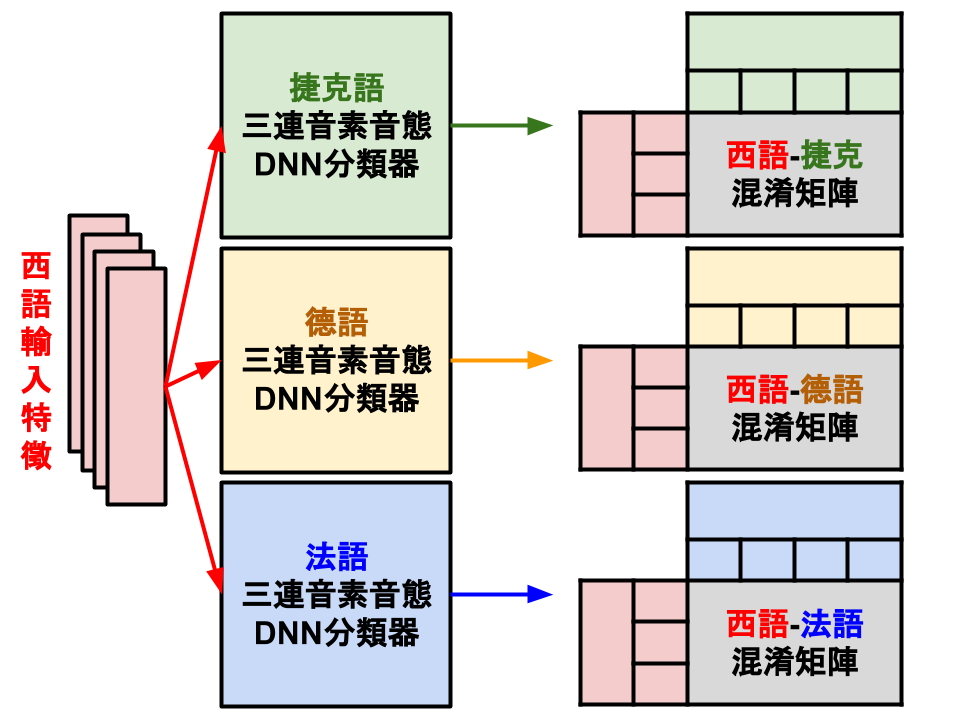
\includegraphics[scale=0.4]{images/chap4_cross_decode.png}
\caption{針對西班牙語言的輸入特徵向量,分別以單語言類神經網路分類器進行捷克語、德語以及法語的交叉解碼(Cross Decode),以計算非對稱混淆矩陣。}
\label{fig:chap4_cross_decode}
\end{figure}

在語音辨識系統中,特定語言語料所訓練的深層類神經網路模型用於給定輸入另一種語言的特徵向量,分類前者的三連音素狀態,如圖\ref{fig:chap4_cross_decode}。如果對西班牙語的輸入特徵向量使用訓練於德語的深層類神經網路進行分類時,即可以得到實際類別為西班牙語三連音素狀態集、預測類別為德語三連音素狀態集的混淆矩陣。依此推類,總計可以產生12組非對稱的混淆矩陣,如公式(\ref{eq:chap4_CM_hard})。
\begin{equation} \label{eq:chap4_CM_hard}
M( s^{(l1)} , s^{(l2)} ) = \sum_{ \bold{x} \in D(s^{l1}) } \mathbbm{1} \{ s^{(l2)} = \arg\max_{i} y_{i}^{(l2)}(\bold{x}) \}
\end{equation}
其中$s^{(l1)}$、$s^{(l2)}$分別是來自語言l1和l2的三連音素狀態,$D(s^{l1})$是語言l1中實際類別為$s^{(l1)}$的輸入訓練特徵向量集,$y_{i}^{(l2)}(\bold{x})$是語言l2的深層類神經網路分類器,在輸入特徵向量$\bold{x}$後,最後一層軟性最大化輸出層的第i維。$\mathbbm{1}\{ \}$ 為指示函數(Indicator Function),當輸入邏輯為真的時候,函數輸出為1,反之則為0。

以深層類神經網路模型進行跨語言分類時,分類器並沒有正確答案,因為本來就屬於不同語言的範疇。但某一項分類的機率越高,代表的是兩個三連音素狀態的近似程度越高。公式(\ref{eq:chap4_CM_hard})使用的是如傳統混淆矩陣的硬式預測(Hard Predicion),但為了得到更豐富的混淆度,可以使用如公式\ref{eq:chap4_CM_soft}的軟式預測(Soft Prediction),把模型分類的機率直接納入考量,而不只是考量最大值,納入較多資訊。
\begin{equation} \label{eq:chap4_CM_soft}
M( s^{(l1)} , s^{(l2)} ) = \sum_{ \bold{x} \in D(s^{l1}) } y_{i}^{(l2)}(\bold{x}) 
\end{equation}

有了軟式混淆矩陣,再除以實際音素的數量,即可以獲得非對稱的相似度(Asymmetric Similarity),如式\ref{eq:chap4_asym_sim}。
\begin{equation} \label{eq:chap4_asym_sim}
ASIM( s^{(l1)} , s^{(l2)} ) =  \frac{ M( s^{(l1)} , s^{(l2)}) } { count( s^{(l1)} )}
\end{equation}

每對不同語言的三連音素狀態,會有兩個混淆矩陣算出來的非對稱相似度,如公式\ref{eq:chap4_sym_sim}平均後,即為這兩個三連音素狀態的對稱相似度(Symmertric Similarity)。
\begin{equation} \label{eq:chap4_sym_sim}
SIM( s^{(l1)} , s^{(l2)} ) =  \frac{ ASIM( s^{(l1)} , s^{(l2)})  + ASIM( s^{(l2)} , s^{(l1)})} {2 }
\end{equation}
\subsection{階層式累積分群合併}

階層式累積分群(Hierarchical Agglomerative Clustering, HAC)是一個非監督式分群方法,給定各個訓練實例在空間中的距離,由下而上合併實例,最後停在足夠概括的分群設定下。演算法設定與步驟如下:

\begin{itemize}
 \itemsep -2pt
 \item 計算語言間所有三連音素狀態之間的對稱相似度,如公式\ref{eq:chap4_sym_sim}。
 \item 找出相似度最高的一對三連音素狀態$( s^{(l1)} , s^{(l2)}  )$。
 \item 如果這組三連音素狀態已經合併過,或是合併後會導致有同語言的三連音素狀態被合併在一起,則不合併這組。
 \item 持續找出最大的相似度並且合併三連音素狀態,直到合併到指定的三連音素狀態數量。
\end{itemize}

如圖\ref{fig:chap4_hac},同一語言的三連音素狀態,在訓練聲學模型時就已經強制分開,因此在階層式分群合併跨語言音素時,不會再進行合併。

\begin{figure}[!h]
\centering
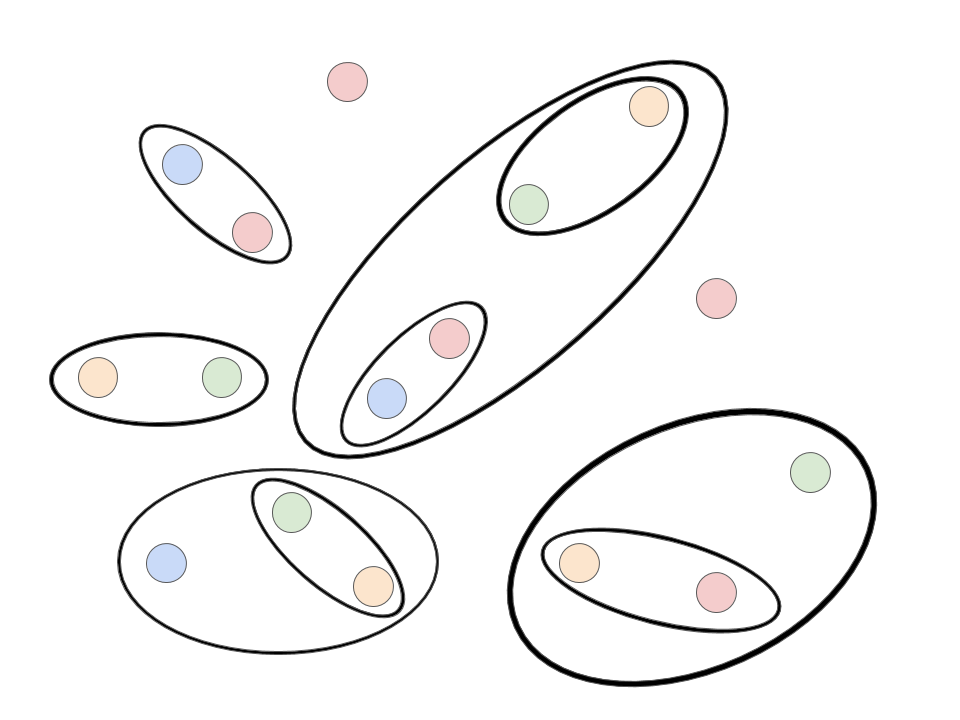
\includegraphics[scale=0.4]{images/chap4_hac.png}
\caption{階層式累積分群合併示意圖。圖中不同顏色的原點代表四個語言的三連音素狀態分佈在空間中,黑色圈圈為合併的結果。合併過程會優先將鄰近的音素狀態合併起來,但不會將同一個語言的音素狀態合併,因此每一群最多只會有四個原點。}
\label{fig:chap4_hac}
\end{figure}


\begin{table}[!h]
%\resizebox{\columnwidth}{!}{
\centering
\begin{tabular}{|cccc|}
\hline
\# & 相似度   & 三連音素狀態    & 三連音素狀態    \\
\hline
2  & 0.691 & 捷克753(s)  & 西語690(s)  \\
\hline
12 & 0.571 & 法語579(S)  & 德語1051(z) \\
\hline
16 & 0.558 & 法語580(AE) & 德語1048(x) \\
\hline
19 & 0.541 & 法語1407(a) & 西語187(a) \\
\hline
\end{tabular}
\caption{基於混淆矩陣合併三連音素狀態,第一行為合併的優先序。三連音素狀態除了編號之外,括號內顯示其中間音素。}
\label{table:chap4_CM_merge_examples}
\end{table}
表\ref{table:chap4_CM_merge_examples}為合併的實例。為了語音辨識系統穩健性,通常會在發音單位中加上沉默(Silence, sil)當作一種音素,儘管他意味著不發音。大部分的合併都是沉默狀態的合併,不列在表上。從表格看來,基於混淆矩陣合併三連音素狀態,其中間的音素在語言學上亦是接近的單位,如法語的S與德語的z。但實際上合併的則是法語編號579以及德語編號1051的三連音素狀態,比音素細緻且人耳無法辨識。

從表\ref{table:chap4_CM_merge_examples}中可以看到如順序16,法語的580以及德語的1048,兩個三連音素狀態的中間音素並不相似,在語言學無法解釋其資料的相似性。

\subsection{合併三連音素狀態的多語言語音辨識系統}

基於混淆矩陣合併好三連音素狀態,整體的系統架構如圖\ref{fig:chap4_CM_framework}。在訓練單語言語音辨識系統時,每個語言會先訓練單連音素狀態與三連音素狀態的聲學模型。但在訓練深層類神經網路聲學模型時,會把四個語言的三連音素狀態合併起來訓練,形成多語言語音辨識系統。
\begin{figure}[!h]
\centering
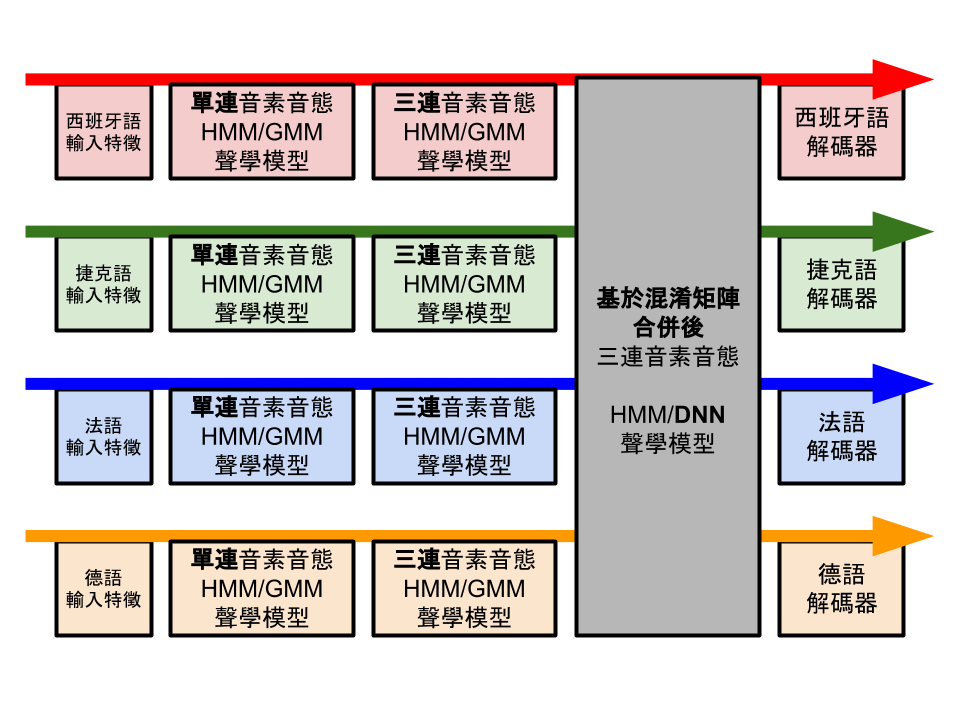
\includegraphics[scale=0.4]{images/chap4_CM_merged.png}
\caption{基於混淆矩陣合併三連音素狀態,多語言語音辨識系統訓練架構圖。其中每個語言訓練的前兩個階段,與單語言語音辨識系統相同。}
\label{fig:chap4_CM_framework}
\end{figure}

經過階層式合併,原本屬於各自語言的三連音素狀態,會與相近的其他語言三連音素狀態合併,再由深層類神經網路模型去預測合併後的類別,形成如圖\ref{fig:chap4_CM_merged_unit}的分類器架構。深層類神經網路輸出的最後一層邏輯子,會以跨語言三連音素狀態的方式訓練,但會在解碼時對應回該特定語言的三連音素狀態,形成包含多語言知識的單語言語音辨識解碼器。
\begin{figure}[!h]
\centering
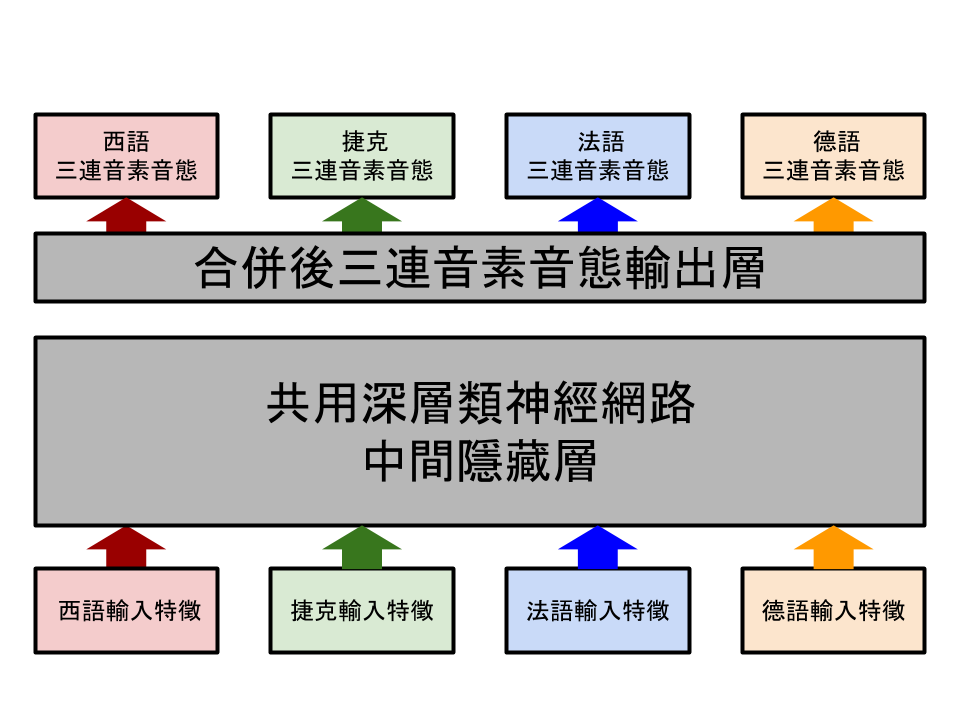
\includegraphics[scale=0.4]{images/chap4_CM_merged_unit}
\caption{基於混淆矩陣合併三連音素狀態,多語言語音辨識系統的深層類神經網路訓練示意圖。}
\label{fig:chap4_CM_merged_unit}
\end{figure}

\subsection{加上國際音標限制}
基於國際音標合併發音單位的方式,是純粹基於語言學上的知識,但只能提供較粗的音素層級的合併;基於混淆矩陣合併三連音素狀態的方式,是純粹考量資料分佈的混淆程度,誤差會干擾其中的結果。圖\ref{fig:chap4_CM_IPA}為法語與西語間的混淆矩陣。

\begin{figure}[!h]
\centering
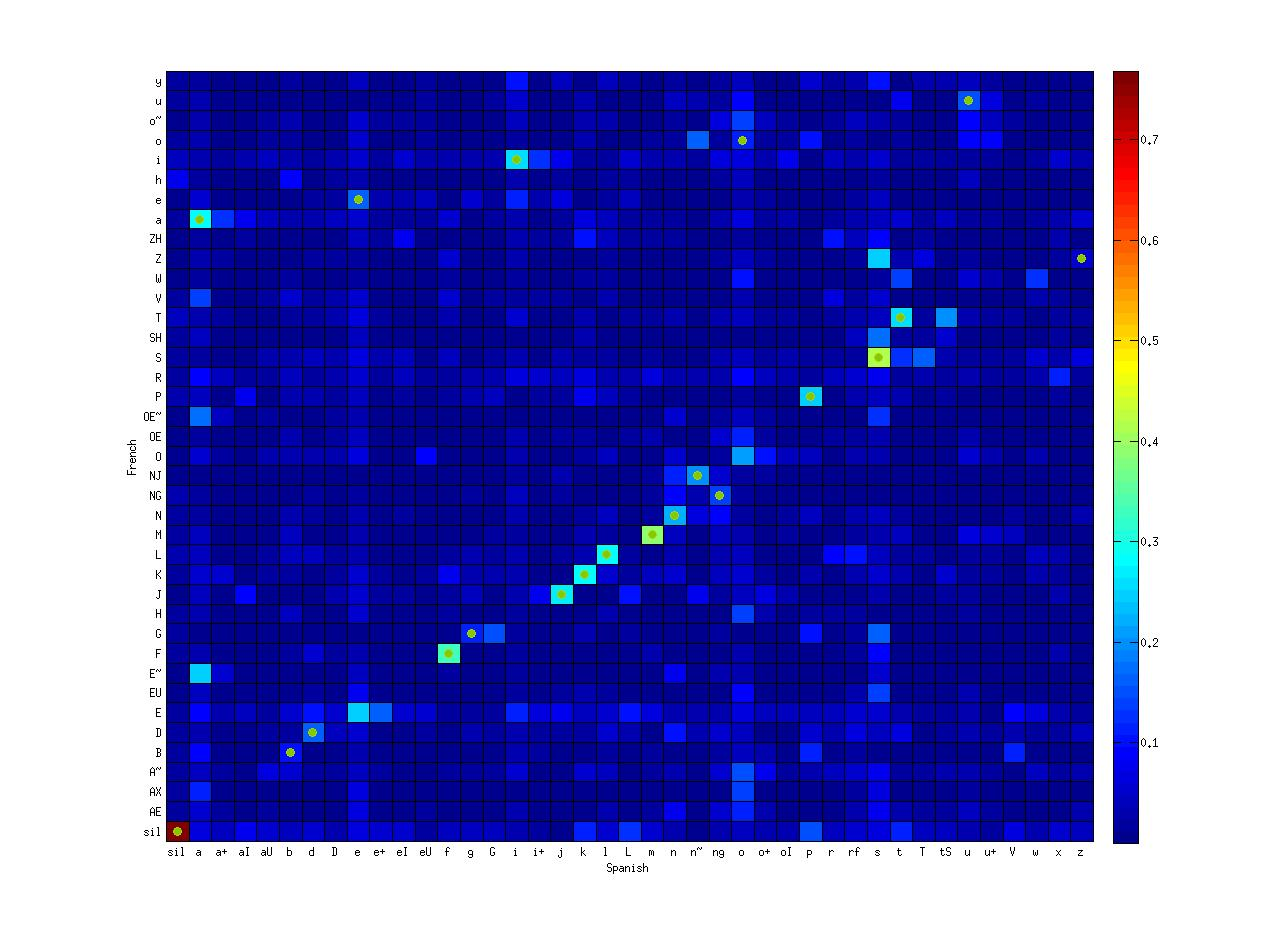
\includegraphics[scale=0.3]{images/chap4_CM_IPA}
\caption{法語對於西語的非對稱相似度混淆矩陣,合併成音素層級。橫軸是法語的音素,縱軸是西語的音素。矩陣元素的顏色代表相似度的值,越深藍越低,越黃紅越高。綠色圓點代表國際音標屬於同一個符號的組合。左下角的沉默音素顯然擁有極高的相似度。}
\label{fig:chap4_CM_IPA}
\end{figure}

為了方便理解發音單位之間的關聯,圖\ref{fig:chap4_CM_IPA}將三連音素狀態根據中央音素合併為較粗的音素單位呈現,綠色的圓點代表兩個音素在國際音標中被標定為相同的符號。

圖\ref{fig:chap4_CM_IPA}中大部份的顏色偏藍色系,代表的是混淆度不高,即大部分的音素彼此不容易混淆;然而顏色偏亮偏黃的,即為資料混淆度較高的音素。由圖中可知,混淆程度高的部份大致和國際音標的合併趨勢相符,但混淆矩陣仍明顯顯示在有些音素對應關係中呈現高混淆度。

如果純粹基於混淆矩陣合併三連音素狀態,雖然能夠合併比較細緻的發音單位,卻缺少了語言學的限制,有可能將不合理的發音單位合併起來。

為了避免誤差影響合併結果,在合併三連音素狀態時,可以在階層式分群時加入語言知識的限制,亦即當兩個三連音素狀態的中央音素不屬於同一個國際音標符號,兩狀態就不能合併。

\subsection{實驗結果與分析}

\begin{table}[htbp]
%\resizebox{\columnwidth}{!}{
\centering
\begin{tabular}{|c>{\columncolor{red!20}}c>{\columncolor{green!20}}c>{\columncolor{blue!20}}c>{\columncolor{yellow!20}}c>{\columncolor{gray}}cc|}
\hline
 方法 & 西語 & 捷克 & 法語 & 德語 & AWERR & 參數數量 \\
\hline
  (1) 單語言基準實驗 & 8.74\% & 18.16\% & 17.43\% & 15.85\% & 100\% & 75.6M \\
\hline
  (2) 國際音標(6073) & 10.03\% & 18.89\% & 18.78\% & 17.27\% & 108.8\% & 26.3M \\
\hline
  (3) 混淆矩陣(6073) & 8.78\% & 18.01\% & 17.54\% & 14.75\% & 98.28\% & 26.3M \\
  (4) +國際音標限制 & 8.83\% & 18.09\% & 17.66\% & 16.06\% & 100.82\% & 26.3M \\
\hline
  (5) 國際音標(7633) & 9.53\% & 19.13\% & 18.60\% & 17.08\%  & 107.2\% & 29.5M\\
\hline
  (6) 混淆矩陣(7633) & 8.67\% & 17.89\% & 17.50\% & 15.16\%  & 98.42\% & 29.5M\\
\hline
  (7) 國際音標(8010) & 9.51\% & 18.80\% & 18.56\% & 16.78\%  & 106.2\% & 30.3M\\
\hline
  (8) 混淆矩陣(8010) & 8.87\% & 17.82\% & 17.68\% & 15.32\%  & 99.4\% & 30.3M\\
\hline
\end{tabular}
\caption{基於混淆矩陣合併三連音素狀態之多語言語音辨識系統,與基準實驗還有國際音標合併的實驗比較。括號內是合併後的三連音素狀態數量。表中的聲學模型都是使用S型函數深度4層,寬度為2048神經元的深層類神經網路。(1)為表\ref{table:chap3_dropout}中使用S型函數的基準實驗,為計算AWERR的基準。(2)(5)(7)為表\ref{table:chap4_IPA_merged}中合併國際音標實驗中,不同音素狀態設定的結果。(3)(6)(8)為本節使用混淆矩陣合併音素狀態後的結果,刻意設定與國際音素合併的設定相同,以方便比較。(4)為實驗(3)的設定下,額外添加國際音標限制。}
\label{table:chap4_CM_merged}
\end{table}

表\ref{table:chap4_CM_merged}為實驗結果,為了控制在相同的參數數量方便比較結果,在階層式分群時,設定合併的三連音素狀態的數量與表\ref{table:chap4_IPA_merged}相同。

表中可以看到,基於混淆矩陣合併三連音素狀態(3)(6)(8),不僅整體的表現都比單語言語音辨識系統(1)好,參數數量也跟國際音標合併的深層類神經網路(2)(5)(7)一樣。這個方法成功借助其他語言的資訊,輔助本身語言的學習,藉由合併細緻的三連音素狀態,提升資料量。

此外,表\ref{table:chap4_IPA_merged}中可以看到,在基於混淆矩陣合併三連音素狀態時,如果加上國際音標的限制如實驗(4),都沒有使得結果變得更好。這表示語言知識的限制反而干擾了資料混淆矩陣所呈現的相似度,使得階層式分群時較難將相近的三連音素狀態合併起來,共享深層類神經網路訓練。

由這些結果可知,基於混淆矩陣合併三連音素狀態的多語言語音辨識系統,可以成功降低詞錯誤率以及參數數量,利用模型共享增加資料量,幫助深層類神經網路聲學模型學習。相比於基於國際音標合併音素的多語言語音辨識系統,成功的原因在於找出更細緻的發音單位合併方式。

\section{基於模型共享的中間層合併}
\subsection{深層神經網路中間層合併}
鑒於合併三連音素狀態的成功,更深入的研究在於如何找到更細緻的合併方式。以深層類神經網路模型作為三連音素狀態分類器的過程中,中間的隱藏層在訓練過程,由淺至深逐漸學習到時頻資訊以及語音資訊,在最後一層的時候,輔助三連音素狀態的分類。

因此,如果將合併層級,從分類器最後輸出層的三連音素狀態,往前推移到更細緻的深層類神經網路中間層,而讓最後一層分類器能夠根據不同語言有不同的輸出層。

藉由共享深層類神經網路模型的中間層,可以讓模型學習到跨語言的聲音資訊,形成跨語言特徵萃取器,與各語言的專屬三連狀態分類器,同時訓練,如圖\ref{fig:chap4_dnn_sharing}。
\begin{figure}[!h]
\centering
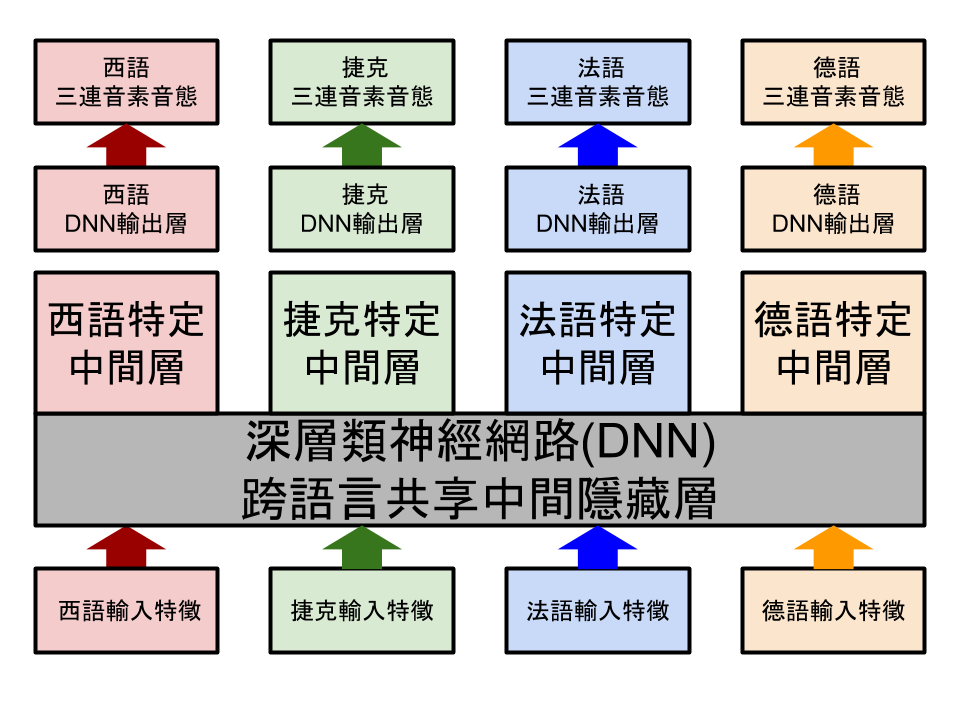
\includegraphics[scale=0.4]{images/chap4_dnn_sharing.png}
\caption{基於模型共享的中間層合併,多語言語音辨識系統中的深層類神經網路模型訓練示意圖。模型的輸出層並沒有合併發音單位,只合併模型前端中間層的參數。}
\label{fig:chap4_dnn_sharing}
\end{figure}

但深層類神經網路模型的參數非常多,一層一層疊加,中間層到底學到什麼樣的資訊,都是在反向傳播過程中自動學習而成,無法分析得知,有不少學者亦致力於其中研究\cite{nagamine2015exploring}。因此,在共享時,哪些中間層該共享學習,是核心的關鍵。

深層類神經網路模型中,越靠近輸入端的中間層,越是能夠學習底層訊號端的知識,其中包含人類語音訊號的頻譜特徵。對於這個底層資訊,有兩種可能的假設:
\begin{itemize}
 \itemsep -2pt
 \item 如果這個底層資訊與語言特色高度相關,共用參數會讓模型受其他語言的資料影響與混淆.訓練效果不彰。分別使用不同的參數,才有足夠的模型能耐學習到語言專屬特色,如圖\ref{fig:chap4_dnn_input_nonsharing}。
 \item 如果這個底層資訊橫跨語言,包含的是語言間共同的頻譜資訊,共用參數會讓模型獲得更加概括化的能力,不僅能降噪,亦能成為很好的特徵萃取器,如圖\ref{fig:chap4_dnn_input_sharing}。
\end{itemize}

\begin{figure}[!h]
\centering
\subfloat[][輸入層不共享] {
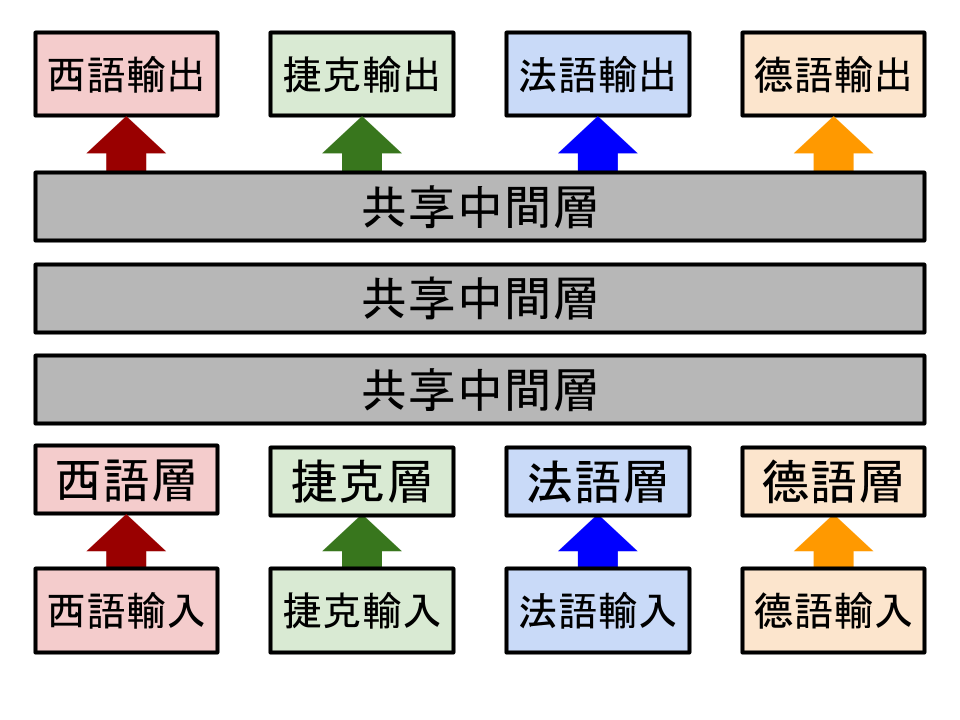
\includegraphics[scale=0.18]{images/chap4_dnn_input_nonsharing.png}
\label{fig:chap4_dnn_input_nonsharing}
}
\subfloat[][全部共享] {
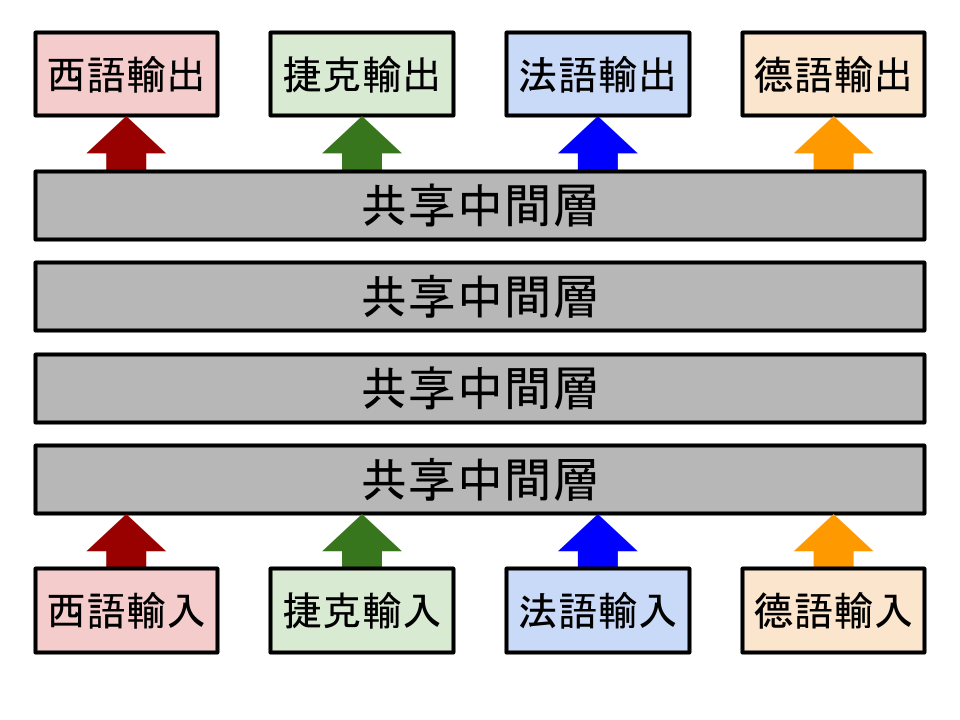
\includegraphics[scale=0.18]{images/chap4_dnn_input_sharing.png}
\label{fig:chap4_dnn_input_sharing}
}
\caption{基於模型共享的中間層合併,兩種可能共享設定。}
\end{figure}

模型中越靠近輸出端的中間層,包含的是高階的語言專屬知識,以提供分類器區分三連音素狀態。
\subsection{實驗結果與比較}

\begin{table}[htbp]
%\resizebox{\columnwidth}{!}{
\centering
\caption{基於模型共享的中間層合併,多語言語音辨識系統的實驗結果。表中的聲學模型都是使用S型函數深度4層,寬度為2048神經元的深層類神經網路。}
\label{table:chap4_dnn_sharing_baseline}
\begin{tabular}{|c>{\columncolor{red!20}}c>{\columncolor{green!20}}c>{\columncolor{blue!20}}c>{\columncolor{yellow!20}}c>{\columncolor{gray}}cc|}
\hline
 方法 & 西語 & 捷克 & 法語 & 德語 & AWERR & 參數數量 \\
\hline
  單語言基準實驗 & 8.74\% & 18.16\% & 17.43\% & 15.85\% & 100\% & 75.6M \\
\hline
  輸入層不共享 & 8.90\% & 18.09\% & 17.69\% & 15.32\% & 99.88\% & 40.2M \\
\hline
  中間層全部共享 & 8.50\% & 17.73\% & 18.05\% & 14.28\% & 97.02\% & 36.4M \\
%\hline
%  輸出層前兩層不共享 & 8.72\% & 18.16\% & 18.61\% & 14.75\%  & 99.78\% & 49.0M\\
\hline
\end{tabular}
\end{table}

表\ref{table:chap4_dnn_sharing_baseline}為模型共享的基準實驗,與單語言語音辨識系統的結果比較。輸入層不共享的結果比全部共享來得較差,表示靠近輸入層的中間層應包含跨語言的頻譜知識,進行跨語言訓練能夠增加資料量幫助訓練。

%原本預期靠近輸出層的中間層富含較多的語言特定知識,但從表\ref{table:chap4_dnn_sharing_baseline}中的結果顯示,輸出層前兩層不共享的結果比全部中間層共享的結果差,推測是深度不足,4層的資訊如果共用仍然能學到更多的東西。

\begin{table}[htbp]
%\resizebox{\columnwidth}{!}{
\centering
\begin{tabular}{|c>{\columncolor{red!20}}c>{\columncolor{green!20}}c>{\columncolor{blue!20}}c>{\columncolor{yellow!20}}c>{\columncolor{gray}}cc|}
\hline
 方法 & 西語 & 捷克 & 法語 & 德語 & AWERR & 參數數量 \\
\hline
  (1)單語言4層基準實驗 & 8.74\% & 18.16\% & 17.43\% & 15.85\% & 100\% & 75.6M \\
  (2)+線性整流與丟棄0.1 & 8.58\% & 17.61\% & 17.15\% & 15.40\% & 97.67\% & 75.6M \\
  (3)+增加至7層中間層 & 8.41\% & 17.03\% & 16.80\% & 14.50\% & 94.45\% & 128.3M \\
\hline
  (4)4層共享中間層 & 8.50\% & 17.73\% & 18.05\% & 14.28\% & 97.02\% & 36.4M \\
  (5)+線性整流與丟棄0.1 & 8.29\% & 17.05\% & 16.93\% & 14.15\% & 93.74\% & 36.4M \\
  (6)+增加至7層共享中間層 & 8.10\% & 16.75\% & 16.65\% & 12.95\% & 90.38\% & 49.9M \\
%\hline
%  前4層共享+後3層不共享 & 7.96\% & 16.56\% & 16.42\% & 13.57\%  & 90.47\% & 86.8M\\
\hline
\end{tabular}
\caption{基於模型共享的中間層合併,多語言語音辨識系統的實驗結果。表中的聲學模型都是使用寬度為2048神經元的深層類神經網路。}
\label{table:chap4_dnn_sharing}
\end{table}
表\ref{table:chap4_dnn_sharing}將單語言基準實驗時的丟棄演算法加入比較,並且增加深度,結果與表\ref{table:chap3_dropout}和表\ref{table:chap3_depth}一致,使用丟棄演算法和增加深度都能使結果變好,但仍需要注意到參數數量的提升。
\section{本章實驗比較與綜合分析}
\begin{table}[]
%\resizebox{\columnwidth}{!}{
\centering
\begin{tabular}{|c|c|c|c|c|}
\hline
\multirow{2}{*}{方式} & \multirow{2}{*}{AWERR}    & 是否合併& 是否合併             & 是否合併 \\
     & & DNN  & 三連音素狀態 &  聲學模型轉移模型 \\
\hline
單語言基礎實驗  & 100\% &  &  &   \\
\hline
(1) 基於國際音標 & \multirow{2}{*}{106.2\% } & \multirow{2}{*}{ 是 } & \multirow{2}{*}{是}  & \multirow{2}{*}{是}  \\
合併音素& & & & \\
\hline
(2) 基於混淆矩陣 & \multirow{2}{*}{ 98.28\%} & \multirow{2}{*}{ 是 } & \multirow{2}{*}{是}  &  \\
合併三連音素狀態& & & & \\
\hline
(3) 基於模型共享 & \multirow{2}{*}{97.02\%} &\multirow{2}{*}{ 是 } &  &  \\
合併中間層 & & & & \\
\hline
\end{tabular}
\caption{本章三種合併發音單位的實驗比較,用以訓練多語言語音辨識系統內的深層類神經網絡模型。表中數據都使用S型函數、深度為4層、寬度為2048神經元的模型中,該方法下最好的AWERR結果,與表\ref{table:chap4_IPA_merged} 8010個狀態、表\ref{table:chap4_CM_merged} 6073個狀態以及表\ref{table:chap4_dnn_sharing_baseline} 全部共享一致。}
\label{table:chap4_merging_illustrator}
\end{table}
多語言語音辨識聲學模型中,深度類神經網路佔據著不可或缺的地位,然其訓練過程需要特別多的資料量,如果能從其他語言中借助更多的資料幫助訓練,增強模型潛力。

然所謂的更多資料,充其量也只是更多充滿雜訊的不匹配資料而已,從機器學習的角度上來看,甚至會干擾模型的學習,必須找到可以合併共享的部分,只學習合適且重要的資訊來達到目標。

本章從音素合併模型,開始逐步磨細成三連音素狀態合併,最後停在深層類神經網路模型的中間層合併,整體的脈絡如表\ref{table:chap4_merging_illustrator},由粗糙到細緻的發音單位合併。

即便人耳最多只能鑑別音素,有許多差異是只有機器才能區別出來。這些橫跨語言的知識,與語言特性高度相關。本研究使用的四個語言都是印歐語系,但是屬於不同分支,因此仍然可以從中看到多語言語音辨識系統架構設計上的蹊蹺。
